%\documentclass[smaller,handout]{beamer}
\def\bmode{0} % Mode 0 for presentation, mode 1 for a handout with notes, mode 2 fo% r handout without notes
\if 0\bmode
\documentclass[smaller]{beamer}
\else \if 1\bmode
\immediate\write18{pdflatex -jobname=\jobname-Handout-Notes\space\jobname}
\documentclass[smaller,handout]{beamer}
\usepackage{handoutWithNotes}
\pgfpagesuselayout{2 on 1 with notes}[letterpaper, landscape, border shrink=4mm]
\else \if 2\bmode
\immediate\write18{pdflatex -jobname=\jobname-Handout\space\jobname}
\documentclass[smaller,handout]{beamer}
\fi
\fi
\fi

%%%%%%%%%%%%%%%%%%%%%%%%%%%%%%%%%%%%%%%%%%%%%%%%%%%%%%%%%%%%%%%%%%%%%%%%%%%%%%%%%%%%%%%%%%%%%
\newcommand{\coursetitle}{CEE 616: Probabilistic Machine Learning}
\newcommand{\longlecturetitle}{M3 Deep Neural Networks:\\ Neural Networks for Structured Data I}
\newcommand{\shortlecturetitle}{L3a: NNs for Structured Data}
\newcommand{\instructor}{Jimi Oke}
\newcommand{\lecturedate}{Thu, Oct 16, 2025}
%%%%%%%%%%%%%%%%%%%%%%%%%%%%%%%%%%%%%%%%%%%%%%%%%%%%%%%%%%%%%%%%%%%%%%%%%%%%%%%%%%%%%%%%%%%%%

 
 
% \usepackage[T1]{fontenc} 
% \usepackage{lmodern} 
%\usepackage{etex}
 %\newcommand{\num}{6{} }

% \usetheme[
%   outer/progressbar=foot,
%   outer/numbering=fraction,
%   block=fill,
%   inner/subsectionpage=progressbar
% ]{metropolis}
\usetheme{Madrid}
\useoutertheme[subsection=false]{miniframes} % Alternatively: miniframes, infolines, split
\useinnertheme{circles}
% %\useoutertheme{Frankfurt}
% \usecolortheme{beaver}
% %\useoutertheme{crane}
% %\useoutertheme{metropolis}
\usepackage[backend=biber,style=authoryear,maxcitenames=2,maxbibnames=99,safeinputenc,url=false, eprint=false]{biblatex}
%\addbibresource{bib/references.bib}
% \AtEveryCitekey{\iffootnote{{\tiny}\tiny}{\tiny}}

% %\usepackage{pgfpages}
% %\setbeameroption{hide notes} % Only slides
% %\setbeameroption{show only notes} % Only notes
% %\setbeameroption{hide notes} % Only notes
% %\setbeameroption{show notes on second screen=right} % Both

% % \usepackage[sfdefault]{Fira Sans}

% % \setsansfont[BoldFont={Fira Sans}]{Fira Sans Light}
% % \setmonofont{Fira Mono}

% %\usepackage{fira}
% %\setsansfont{Fira}
% %\setmonofont{Fira Mono}
% % To give a presentation with the Skim reader (http://skim-app.sourceforge.net) on OSX so
% % that you see the notes on your laptop and the slides on the projector, do the following:
% % 
% % 1. Generate just the presentation (hide notes) and save to slides.pdf
% % 2. Generate onlt the notes (show only nodes) and save to notes.pdf
% % 3. With Skim open both slides.pdf and notes.pdf
% % 4. Click on slides.pdf to bring it to front.
% % 5. In Skim, under "View -> Presentation Option -> Synhcronized Noted Document"
% %    select notes.pdf.
% % 6. Now as you move around in slides.pdf the notes.pdf file will follow you.
% % 7. Arrange windows so that notes.pdf is in full screen mode on your laptop
% %    and slides.pdf is in presentation mode on the projector.

% % Give a slight yellow tint to the notes page
% \setbeamertemplate{note page}{\pagecolor{yellow!5}\insertnote}\usepackage{palatino}

% %\usetheme{metropolis}
% %\usecolortheme{beaver}
 \usepackage{tipa}
% \usepackage{enumerate}
\definecolor{darkcandyapplered}{HTML}{A40000}
\definecolor{lightcandyapplered}{HTML}{e74c3c}

% %\setbeamercolor{title}{fg=darkcandyapplered}

% \definecolor{UBCblue}{rgb}{0.04706, 0.13725, 0.26667} % UBC Blue (primary)
% \definecolor{UBCgrey}{rgb}{0.3686, 0.5255, 0.6235} % UBC Grey (secondary)

% % \setbeamercolor{palette primary}{bg=darkcandyapplered,fg=white}
% % \setbeamercolor{palette secondary}{bg=darkcandyapplered,fg=white}
% % \setbeamercolor{palette tertiary}{bg=darkcandyapplered,fg=white}
% % \setbeamercolor{palette quaternary}{bg=darkcandyapplered,fg=white}
% % \setbeamercolor{structure}{fg=darkcandyapplered} % itemize, enumerate, etc
% % \setbeamercolor{section in toc}{fg=darkcandyapplered} % TOC sections
% % \setbeamercolor{frametitle}{fg=darkcandyapplered,bg=white} % TOC sections
% % \setbeamercolor{title in head/foot}{bg=white,fg=white} % TOC sections
% % \setbeamercolor{button}{fg=darkcandyapplered} % TOC sections

% % % Override palette coloring with secondary
% % \setbeamercolor{subsection in head/foot}{bg=lightcandyapplered,fg=white}

%\usecolortheme{crane}
% \makeatletter
% \setbeamertemplate{headline}{%
%   \begin{beamercolorbox}[colsep=1.5pt]{upper separation line head}
%   \end{beamercolorbox}
%   \begin{beamercolorbox}{section in head/foot}
%     \vskip1pt\insertsectionnavigationhorizontal{\paperwidth}{}{}\vskip1pt
%   \end{beamercolorbox}%
%   \ifbeamer@theme@subsection%
%     \begin{beamercolorbox}[colsep=1.5pt]{middle separation line head}
%     \end{beamercolorbox}
%     \begin{beamercolorbox}[ht=2.5ex,dp=1.125ex,%
%       leftskip=.3cm,rightskip=.3cm plus1fil]{subsection in head/foot}
%       \usebeamerfont{subsection in head/foot}\insertsubsectionhead
%     \end{beamercolorbox}%
%   \fi%
%   \begin{beamercolorbox}[colsep=1.5pt]{lower separation line head}
%   \end{beamercolorbox}
% }
% \makeatother

% Reduce size of frame box
\setbeamertemplate{frametitle}{%
    \nointerlineskip%
    \begin{beamercolorbox}[wd=\paperwidth,ht=2.0ex,dp=0.6ex]{frametitle}
        \hspace*{1ex}\insertframetitle%
    \end{beamercolorbox}%
}


%\setbeamercolor{frametitle}{bg=darkcandyapplered!80!black!90!white}
%\setbeamertemplate{frametitle}{\bf\insertframetitle}

%\setbeamercolor{footnote mark}{fg=darkcandyapplered}
%\setbeamercolor{footnote}{fg=darkcandyapplered!70}
%\Raggedbottom
%\setbeamerfont{page number in head/foot}{size=\tiny}
%\usepackage[tracking]{microtype}


% %\usepackage[sc,osf]{mathpazo}   % With old-style figures and real smallcaps.
% %\linespread{1.025}              % Palatino leads a little more leading

% % Euler for math and numbers
% %\usepackage[euler-digits,small]{eulervm}
% %\AtBeginDocument{\renewcommand{\hbar}{\hslash}}
\usepackage{graphicx}
\usepackage{multirow}
\usepackage{booktabs}
\usepackage{graphbox}
\usepackage{animate}
\usepackage{media9}
\usepackage{adjustbox}

% %\mode<presentation> { \setbeamercovered{transparent} }

\setbeamertemplate{navigation symbols}{}
\makeatletter
\def\beamerorig@set@color{%
  \pdfliteral{\current@color}%
  \aftergroup\reset@color
}
\def\beamerorig@reset@color{\pdfliteral{\current@color}}
\makeatother


% %=== GRAPHICS PATH ===========
\graphicspath{{./m5-images/}}
% % Marginpar width
% %Marginpar width
% %\setlength{\marginparsep}{.02in}


% %% Captions
% % \usepackage{caption}
% % \captionsetup{
% %   labelsep=quad,
% %   justification=raggedright,
% %   labelfont=sc
% % }

% \setbeamerfont{caption}{size=\footnotesize}
% \setbeamercolor{caption name}{fg=darkcandyapplered}

% %AMS-TeX packages

\usepackage{amssymb}
\usepackage{amsmath}
\usepackage{amsthm}
\usepackage{mathtools} 
\usepackage{bm}
\DeclareMathOperator*{\argmax}{arg\,max}
\DeclareMathOperator*{\argmin}{arg\,min}
% \usepackage{color}

% %https://tex.stackexchange.com/a/31370/2269
\usepackage{cancel}
\renewcommand{\CancelColor}{\color{red}} %change cancel color to red
\makeatletter
\let\my@cancelto\cancelto %copy over the original cancelto command
\newcommand<>{\cancelto}[2]{\alt#3{\my@cancelto{#1}{#2}}{\mathrlap{#2}\phantom{\my@cancelto{#1}{#2}}}}
% redefine the cancelto command, using \phantom to assure that the
% result doesn't wiggle up and down with and without the arrow
\makeatother


% % \usepackage{comment}
\usepackage{enumerate}
\usepackage{hyperref}
% \usepackage{minitoc,array}
% \definecolor{slblue}{rgb}{0,.3,.62}
\hypersetup{
    colorlinks,%
    citecolor=blue,%
    filecolor=blue,%
    linkcolor=blue,
    urlcolor=blue
}

% \usepackage{epstopdf}
% \epstopdfDeclareGraphicsRule{.gif}{png}{.png}{convert gif:#1 png:\OutputFile}
% \AppendGraphicsExtensions{.gif}

% %\usepackage{listings}

% %%% TIKZ
\usepackage{forest}
\usepackage{tikz}
\usepackage{tikz-3dplot}
\usepackage{pgfplots}
\usepackage{pgfplotstable}
% \usepackage{pgfgantt}
\usepackage{neuralnetwork}

\usetikzlibrary{fit,arrows,arrows.meta,shapes,positioning,shapes.geometric}
\usetikzlibrary{decorations.markings}
\usetikzlibrary{shadows,automata}
\usetikzlibrary{patterns}
\usetikzlibrary{trees,mindmap,backgrounds}
%\usetikzlibrary{circuits.ee.IEC}
\usetikzlibrary{decorations.text}
% % For Sagnac Picture
% \usetikzlibrary{%
%     decorations.pathreplacing,%
%     decorations.pathmorphing%
% }
% \tikzset{no shadows/.style={general shadow/.style=}}
% %
% %\usepackage{paralist}

\tikzset{
  font=\Large\sffamily\bfseries,
  red arrow/.style={
    midway,red,sloped,fill, minimum height=3cm, single arrow, single arrow head extend=.5cm, single arrow head indent=.25cm,xscale=0.3,yscale=0.15,
    allow upside down
  },
  black arrow/.style 2 args={-stealth, shorten >=#1, shorten <=#2},
  black arrow/.default={1mm}{1mm},
  tree box/.style={draw, rounded corners, inner sep=1em},
  node box/.style={white, draw=black, text=black, rectangle, rounded corners},
}

% %%% FORMAT PYTHON CODE
% %\usepackage{listings}
% % Default fixed font does not support bold face
% \DeclareFixedFont{\ttb}{T1}{txtt}{bx}{n}{8} % for bold
% \DeclareFixedFont{\ttm}{T1}{txtt}{m}{n}{8}  % for normal

% % Custom colors
% \definecolor{deepblue}{rgb}{0,0,0.5}
% \definecolor{deepred}{rgb}{0.6,0,0}
% \definecolor{deepgreen}{rgb}{0,0.5,0}

% %\usepackage{animate}

% % Python style for highlighting
% % \newcommand\pythonstyle{\lstset{
% % language=Python,
% % basicstyle=\footnotesize\ttm,
% % otherkeywords={self},             % Add keywords here
% % keywordstyle=\footnotesize\ttb\color{deepblue},
% % emph={MyClass,__init__},          % Custom highlighting
% % emphstyle=\footnotesize\ttb\color{deepred},    % Custom highlighting style
% % stringstyle=\color{deepgreen},
% % frame=tb,                         % Any extra options here
%     % showstringspaces=false            % 
% % }}

% % % Python environment
% % \lstnewenvironment{python}[1][]
% % {
% % \pythonstyle
% % \lstset{#1}
% % }
% % {}

% % % Python for external files
% % \newcommand\pythonexternal[2][]{{
% % \pythonstyle
% % \lstinputlisting[#1]{#2}}}

% % Python for inline
% % 
% % \newcommand\pythoninline[1]{{\pythonstyle\lstinline!#1!}}

% %\usepackage{algorithm2e}

\newcommand{\eps}{\epsilon}
\newcommand{\bX}{\mb X}
\newcommand{\by}{\mb y}
\newcommand{\bbe}{\bm\beta}
\newcommand{\beps}{\bm\epsilon}
\newcommand{\bY}{\mb Y}

\newcommand{\osn}{\oldstylenums}
\newcommand{\dg}{^{\circ}}
\newcommand{\lt}{\left}
\newcommand{\rt}{\right}
\newcommand{\pt}{\phantom}
\newcommand{\tf}{\therefore}
\newcommand{\?}{\stackrel{?}{=}}
\newcommand{\fr}{\frac}
\newcommand{\dfr}{\dfrac}
\newcommand{\ul}{\underline}
\newcommand{\tn}{\tabularnewline}
\newcommand{\nl}{\newline}
\newcommand\relph[1]{\mathrel{\phantom{#1}}}
\newcommand{\cm}{\checkmark}
\newcommand{\ol}{\overline}
\newcommand{\rd}{\color{red}}
\newcommand{\bl}{\color{blue}}
\newcommand{\pl}{\color{purple}}
\newcommand{\og}{\color{orange!90!black}}
\newcommand{\gr}{\color{green!40!black}}
\newcommand{\lbl}{\color{CornflowerBlue}}
\newcommand{\dca}{\color{darkcandyapplered}}
\newcommand{\nin}{\noindent}
\newcommand*\circled[1]{\tikz[baseline=(char.base)]{
            \node[shape=circle,draw,thick,inner sep=1pt] (char) {\small #1};}}

\newcommand{\bc}{\begin{compactenum}[\quad--]}
\newcommand{\ec}{\end{compactenum}}

\newcommand{\p}{\partial}
\newcommand{\pd}[2]{\frac{\partial{#1}}{\partial{#2}}}
\newcommand{\dpd}[2]{\dfrac{\partial{#1}}{\partial{#2}}}
\newcommand{\pdd}[2]{\frac{\partial^2{#1}}{\partial{#2}^2}}
\newcommand{\pde}[3]{\frac{\partial^2{#1}}{\partial{#2}\partial{#3}}}
\newcommand{\nmfr}[3]{\Phi\left(\frac{{#1} - {#2}}{#3}\right)}
\newcommand{\Err}{\text{Err}}
\newcommand{\err}{\text{err}}

\DeclarePairedDelimiter\ceil{\lceil}{\rceil}
\DeclarePairedDelimiter\floor{\lfloor}{\rfloor}

%%%% GREEK LETTER SHORTCUTS %%%%%
\newcommand{\la}{\lambda}
\renewcommand{\th}{\theta}
\newcommand{\al}{\alpha}
\newcommand{\G}{\Gamma}
\newcommand{\si}{\sigma}
\newcommand{\Si}{\Sigma}


\pgfmathdeclarefunction{poiss}{1}{%
  \pgfmathparse{(#1^x)*exp(-#1)/(x!)}%
  }

\pgfmathdeclarefunction{gauss}{2}{%
  \pgfmathparse{1/(#2*sqrt(2*pi))*exp(-((x-#1)^2)/(2*#2^2))}%
}

\pgfmathdeclarefunction{expo}{2}{%
  \pgfmathparse{#1*exp(-#1*#2)}%
}

\pgfmathdeclarefunction{expocdf}{2}{%
  \pgfmathparse{1 -exp(-#1*#2)}%
}

\newcommand{\mb}{\mathbb}
\newcommand{\mc}{\mathcal}
\newcommand{\tr}{^{\top}}
\newcommand{\empt}[2]{$#1^{( #2 )}$}
\newcommand{\pe}{\pause}
% \usepackage{pst-plot}

% \usepackage{pstricks-add}
% \usepackage{auto-pst-pdf}   

% \psset{unit = 3}

% \def\target(#1,#2){%
%  {\psset{fillstyle = solid}
%   \rput(#1,#2){%
%     \pscircle[fillcolor = white](0.7,0.7){0.7}
%     \pscircle[fillcolor = blue!60](0.7,0.7){0.5}
%     \pscircle[fillcolor = white](0.7,0.7){0.3}
%     \pscircle[fillcolor = red!80](0.7,0.7){0.1}}}}
% \def\dots[#1](#2,#3){%
%     \psRandom[
%       dotsize = 2pt,
%       randomPoints = 25
%     ](!#2 #1 0.04 sub sub #3 #1 0.04 sub sub)%
%      (!#2 #1 0.04 sub add #3 #1 0.04 sub add)%
%      {\pscircle[linestyle = none](#2,#3){#1}}}


%%%%%%%%%%%%%%%%%%%%%%%%%%%%%%%%%%%%%%%%%%%%%%%%%%%
%%%%%%%%%%%%%%%%%%%%%%%%%%%%%%%%%%%%%%%%%%%%%%%%%%%
\title[\shortlecturetitle]{ {\normalsize \coursetitle}
  \\ \longlecturetitle}
\date[\lecturedate]{\footnotesize \lecturedate}
\author{{\bf \instructor}}
\institute[UMass Amherst]{
%\titlegraphic{\hfill
  \begin{tikzpicture}[baseline=(current bounding box.center)]
    \node[anchor=base] at (-7,0) (its) {\includegraphics[scale=.3]{UMassEngineering_vert}} ;
  \end{tikzpicture}
  % \hfill\includegraphics[height=1.5cm]{logo}
}

%https://tex.stackexchange.com/questions/55806/mindmap-tikzpicture-in-beamer-reveal-step-by-step
  \tikzset{
    invisible/.style={opacity=0},
    visible on/.style={alt={#1{}{invisible}}},
    alt/.code args={<#1>#2#3}{%
      \alt<#1>{\pgfkeysalso{#2}}{\pgfkeysalso{#3}} % \pgfkeysalso doesn't change the path
    },
  }


% https://tex.stackexchange.com/questions/446468/labels-with-arrows-for-an-equation
% https://tex.stackexchange.com/a/402466/121799
\newcommand{\tikzmark}[3][]{
\ifmmode
\tikz[remember picture,baseline=(#2.base)] \node [inner sep=0pt,#1](#2) {$#3$};
\else
\tikz[remember picture,baseline=(#2.base)] \node [inner sep=0pt,#1](#2) {#3};
\fi
}

% \lstset{language=matlab,
%                 basicstyle=\scriptsize\ttfamily,
%                 keywordstyle=\color{blue}\ttfamily,
%                 stringstyle=\color{blue}\ttfamily,
%                 commentstyle=\color{gray}\ttfamily,
%                 morecomment=[l][\color{gray}]{\#}
%               }


%%% Local Variables:
%%% mode: latex
%%% TeX-master: t
%%% End:

              
\begin{document}
\maketitle
\begin{frame}
  \frametitle{Outline}
  \tableofcontents
\end{frame}

 
 
 
\section{Introduction}
\begin{frame}
  \frametitle{Neural networks}
  \pe
  Consider the linear model:\pe
  \begin{equation}
    f(\bm x;\bm\th) = \bm w\tr\bm x + \bm b
  \end{equation}\pe
  We can increase the flexibility of the model via a basis function expansion (feature extractor) $\bm\phi(\bm x)$:\pe
  \begin{equation}
    f(\bm x;\bm\th) = \bm W\bm\phi(\bm x) + \bm b
  \end{equation}
  \pe
  If further parameterize $\bm\phi(\bm x)$ by $\bm\th_{2}$ for better fitting, we have:\pe
  \begin{equation}
    f(\bm x;\bm\th) = \bm W\bm\phi(\bm x;\bm\th_{2}) + \bm b
  \end{equation}
  To even further increase complexity, we can recursively fit more feature extractors $f_{\ell}(\bm x;\bm\th_{\ell})$:
  \pe
  \begin{equation}
    f(\bm x;\bm\th) = f_{L}(f_{L-1}(\cdots f_{1}(\bm x;\bm \th_{1}))\cdots))
  \end{equation}
  Each $\ell$ can be considered a layer in a \textbf{feedforward neural network} (FFNN) of $L$ layers.\pe
  \begin{itemize}
  \item Also known as a \textbf{multilayer perception} (MLP)
  \item When $L$ is large, this is termed a \textbf{deep neural network} (DNN)
  \end{itemize}
\end{frame}
\begin{frame}
  \frametitle{Biological neuron}
  \pause


  \visible<2->{\begin{figure}[h!]
    \centering
    \includegraphics[width=.8\textwidth]{neuron}
    \caption{Biological neuron (Source: \url{https://cs231n.github.io/neural-networks-1/})}
  \end{figure}}

  \begin{itemize}[<+->]
  \item $\sim$86 billion neurons are found in the human nervous system
  \item These neurons are connected by 10$^{14}$ to $10^{15}$ synapses
  \item Each neuron receives input signals from its dendrites and outputs signals along a single axon
  \item The axon in turn connects to other neurons via synapses
  \end{itemize}
\end{frame}

\begin{frame}
  \frametitle{Artificial neural networks}
  \pause

  [Artificial] Neural networks (ANNs) are modeled as connected layers of neuron in an acyclic graph (no loops).
  
  \begin{itemize}[<+->]
  \item ANNs are organized into layers of neurons (or ``units'')
  \item Fully-connected layers are common
  \item The basic ANN architecture with multiple hidden layers is called the \textbf{multilayer perceptron (MLP)}
    \begin{itemize}
    \item  An ANN with only one hidden layer is called the \textbf{single layer perceptron}
        \item $N$-layer neural network (number of hidden layers $+$ output layer)
  \end{itemize}
  \item The output neurons have no activation function. Instead, they perform a final transformation of outputs from the penultimate layer
  \end{itemize}
\end{frame}


\begin{frame}
  \frametitle{Computational neuron model}
  \pause
  \begin{figure}[h!]
    \centering

    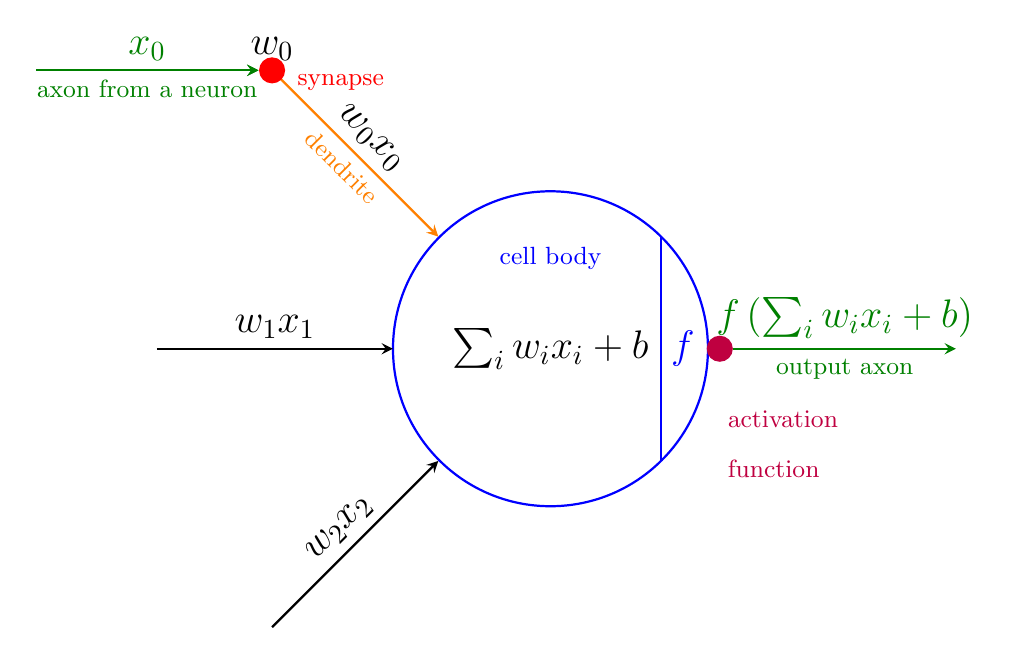
\begin{tikzpicture}[>=stealth,scale=1]
      \visible<13->{\begin{scope}
        \clip[radius=2cm] (0,0) circle;
        \draw[thick,blue] (1.4,-2) -- (1.4,2) node [right,pos=.5] {$f$};
      \end{scope}}
      \visible<12->{\node (O) at (0,0) {$\sum_i w_i x_i + b$ };}
      \visible<11->{\node[above=5mm of O,blue] {\small\normalfont cell body};}
      \visible<10->{\node[blue, thick, draw, circle,minimum width=4cm] at (O) (N) {} ;}
      \visible<14->{\node[circle,fill=purple,minimum width=1mm,xshift=1.5mm] (A) at (2,0) {};}
      \visible<15->{\node[below right of=A,text width=8ex, yshift=-.5cm,purple,] {\small\normalfont activation function};}
      \visible<16->{\draw[->, green!50!black,thick] (A) -- +(3,0) node[below,pos=.5] {\small\normalfont output axon};}
      \visible<17->{\path[->, green!50!black,thick] (A) -- +(3,0) node[above,pos=.5] {$f\lt(\sum_iw_ix_i + b\rt)$};}
      \visible<8->{\draw[->, thick] (-5,0) -- (-2,0) node[above,pos=.5] {$w_1x_1$};}
      \visible<9->{\draw[<-, thick] (N.225) -- (225:5cm) node [above,sloped,pos=.5] {$w_2x_2$};}
      \visible<6->{\draw[<-, thick,orange] (N.135) -- (135:5cm)   node[below,sloped,pos=.5] {\small \normalfont dendrite};}
      \visible<7->{\path[] (N.135) -- (135:5cm)  node[above,sloped,pos=.5] {$w_0x_0$};}
      \visible<4->{\path[] (N.135) -- (135:5cm)  node[opacity=1,circle,fill=red, minimum width=1mm] (W) {};
      \node[above] at (W) (S) {$w_0$};}
      \visible<5->{\node[below right,xshift=2mm,yshift=-2mm] at (S) {\rd \small\normalfont synapse};}
      \visible<2->{\draw[<-, thick,green!50!black ] (135:5cm) (W) -- +(-3,0) node[below,pos=.5] {\small\normalfont axon from a neuron};}
      \visible<3->{\draw[<-, thick,green!50!black ] (135:5cm) (W) -- +(-3,0) node[above,pos=.5] {$x_0$};}
      % \end{scope}
    \end{tikzpicture}
    
    %\caption{Computational neuron components}
  \end{figure}
  
\end{frame}

%\section{Activation functions}
\begin{frame}
  \frametitle{Computational neuron model (cont.)}
  \pause


  \begin{itemize}[<+->]
  \item $x_i$: \pause  signals traveling along axons (inputs)
  \item $w_i$: \pause  measure of synaptic strength, which is learned;\\ \pause
    \begin{itemize}[<+->]\item 
$w_i > 0 \rightarrow$ excitory influence
\item    $w_i <0 \rightarrow$ inhibitory influence
  \end{itemize}
  \item Dendrites carry signals $w_ix_i$ to the cell body, where they are summed.
  \item If the final sum $w_ix_i + b > t$ where $t$ is a threshold\footnote{intercept $b$ is referred to as the ``bias'' in ML literature},
   the neuron sends a spike along its axon (i.e.\ fires)
 \item Computationally, the firing rate of a neuron is represented by an \textbf{\pl activation function $f$}
 \item The output of a neuron is also called the \textit{\pl activation}
  \end{itemize}
\end{frame}

 
 


\begin{frame}[fragile]
  \frametitle{Two-layer neural network (with bias neurons)}
  \begin{figure}[h!]
    \centering
    \begin{neuralnetwork}[height=4 ]
    \newcommand{\x}[2]{$x_#2$}
    \newcommand{\y}[2]{$\hat{y}_#2$}
    \newcommand{\hfirst}[2]{\small $h^{(1)}_#2$}
    \newcommand{\hsecond}[2]{\small $h^{(2)}_#2$}
    \inputlayer[count=3, bias=true, title=I, text=\x]
    \hiddenlayer[count=4, bias=true, title=H1, text=\hfirst] \linklayers
    \outputlayer[count=2, title=O, text=\y] \linklayers
  \end{neuralnetwork}

  \begin{itemize}[<+->]
  \item \textbf{Layers}: 2 (input layer not counted); \pause  \textbf{Hidden layers:} 1
  \item \textbf{Neurons}: 7 (inputs not counted)
  \item \textbf{Learnable parameters:} $(4\times 4) + (5\times 2)$; \pause total = 26
  \end{itemize}
\end{figure}

\end{frame}


 

\begin{frame}[fragile]
  \frametitle{Three-layer neural network (with bias neurons)}
  \begin{figure}[h!]
    \centering
    \begin{neuralnetwork}[height=4]
    \newcommand{\x}[2]{$x_#2$}
    \newcommand{\y}[2]{$\hat{y}_#2$}
    \newcommand{\hfirst}[2]{\small $h^{(1)}_#2$}
    \newcommand{\hsecond}[2]{\small $h^{(2)}_#2$}
    \inputlayer[count=3, bias=true, title=I, text=\x]
    \hiddenlayer[count=4, bias=true, title=H1, text=\hfirst] \linklayers
    \hiddenlayer[count=3, bias=true, title=H2, text=\hsecond] \linklayers
    \outputlayer[count=2, title=O, text=\y] \linklayers
  \end{neuralnetwork}
\end{figure}

\pause
  \begin{itemize}[<+->]
  \item \textbf{Layers}: 3; \pause  \textbf{Hidden layers:} 2
  \item \textbf{Neurons}: 9
  \item \textbf{Learnable parameters:} $(4\times 4) + (5\times 3) + (4\times 2) = \pause 39$ weights; \pause
    total = 39
  \end{itemize}
  
\end{frame}

\section{Activation functions}
\begin{frame}
  \frametitle{Activation functions}
  \pe In an ANN, the activation function $f_{\ell}$ modulates determines whether a certain neuron ``fires'' or passes information (hidden units $\bm z_{\ell}$ at layer $\ell$)
  to the subsequent layer $\ell+1$.\pe
  \begin{equation}
    \bm z_{\ell} = f_{\ell}(\bm z_{\ell-1}) = \varphi_{\ell}(\bm b_{\ell} + \bm W_{\ell}\bm z_{\ell-1})
  \end{equation}
  \begin{itemize}
  \item The input to the activation function $\bm b_{\ell} + \bm W_{\ell}\bm z_{\ell-1}$ is termed the \textbf{pre-activations}:\pe
    \begin{equation}
      \bm a_{\ell}= \bm b_{\ell} + \bm W_{\ell}\bm z_{\ell-1}
    \end{equation}
    \pe
    Thus
    \begin{equation}
      \bm z_{\ell} = \varphi_{\ell}(\bm a_{\ell})
    \end{equation}
  \item In the historic MLP, the activation function was the non-differentiable Heaviside function (difficult to train)
  \item Later on, the sigmoid was introduced (smooth, trainable/differentiable)
    
  \end{itemize}
\end{frame}


\begin{frame}
  \frametitle{Examples of activation functions}
  \pause
  \begin{figure}[t!]
    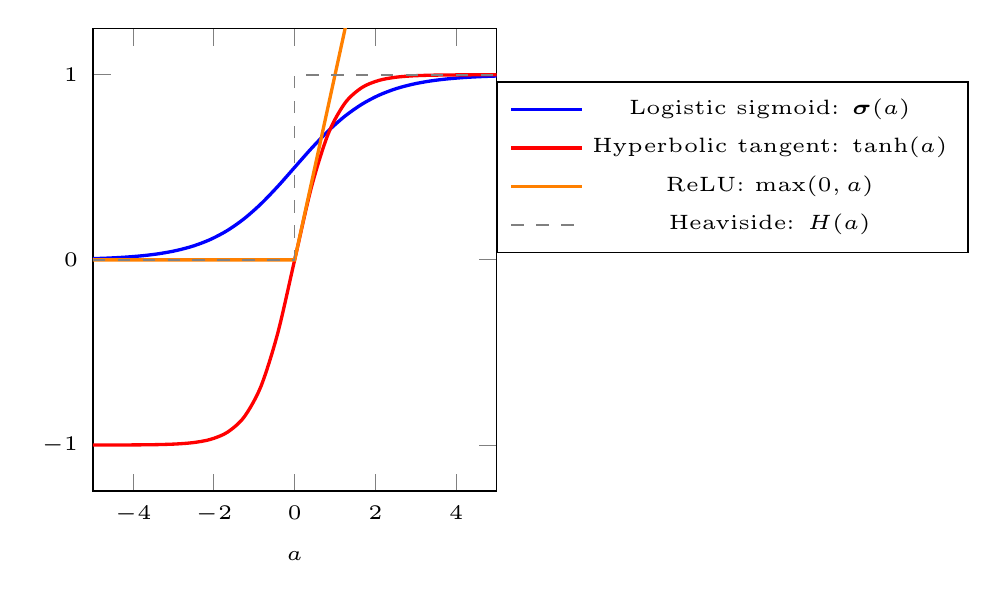
\begin{tikzpicture}[scale=1.5]
      \begin{axis}[width=5cm,height=5.5cm,
        ylabel=,
        xlabel=$a$,ymin=-1.25,ymax=1.25,xmin=-5,xmax=5,
        style={font=\tiny\normalfont},
        legend style ={at={(1,.7)},anchor=west,align=left}
        ]
        \addplot[thick,blue,smooth] {1/(1+exp(-x))}; \addlegendentry{Logistic sigmoid: $\bm\sigma(a)$}
        \addplot[thick,red,smooth] {tanh(x)}; \addlegendentry{Hyperbolic tangent: $\tanh(a)$}
        \addplot[thick,orange,domain=-5:5] {max(0,x)}; \addlegendentry{ReLU: $\max(0,a)$}
%        \addplot[thick,orange,smooth,domain=0:5] {max(0,x)}; 
        \addplot[thin,gray,dashed] coordinates {(-5,0) (0,0) (0,1) (5,1)};
        \addlegendentry{Heaviside: $H(a)$}
      \end{axis}
      \end{tikzpicture}
      
    	% \caption[Sigmoidal activation functions.]{Common used activation functions include the logistic sigmoid $\sigma(z)$ and the hyperbolic tangent $tanh(z)$. More recently used activation functions are the softsign and the rectified hyperbolic tangent.}
    	% \label{fig:sigmoid-tanh}
\end{figure}
\end{frame}

\begin{frame}
  \frametitle{Logistic sigmoid function}
  \begin{itemize}[<+->]
  \item The form of the logistic sigmoid function is given by:
    \begin{equation}
      \bm\sigma(x) = \pause \fr{1}{1 + e^{-x}}
    \end{equation}

  \item It transforms a real-valued input in the interval $[0,1]$.


      \begin{figure}[t!]
    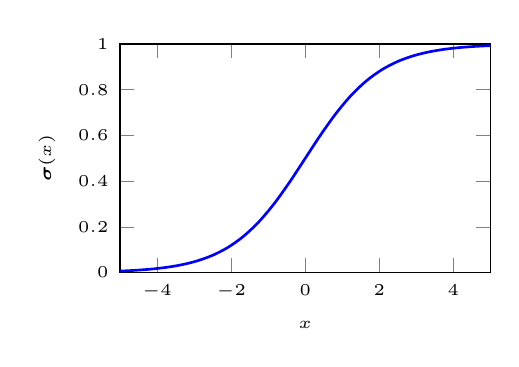
\begin{tikzpicture}[scale=1.2]
      \begin{axis}[width=5.5cm,height=4cm,
        ylabel=$\bm\sigma(x)$,
        xlabel=$x$,ymin=0,ymax=1,xmin=-5,xmax=5,
        style={font=\tiny\normalfont},
        legend style ={at={(0.5,1)},anchor=south,align=left,cells={anchor=left}}
        ]
        \addplot[thick,blue,smooth] {1/(1+exp(-x))};% \addlegendentry{Logistic sigmoid $\sigma(z)$}
        % \addplot[red,smooth] {tanh(x)}; \addlegendentry{Hyperbolic tangent $\tanh(z)$}
        % \addplot[orange,smooth] {1/(1 + abs(x))}; \addlegendentry{Softsign $\fr{1}{1 + |z|}$}          
        % \addplot[green!50!black,smooth] {abs(tanh(x))}; \addlegendentry{Rectified hyperbolic tangent $|\tanh(z)|$}
        \end{axis}
      \end{tikzpicture}
      
    	% \caption[Sigmoidal activation functions.]{Common used activation functions include the logistic sigmoid $\sigma(z)$ and the hyperbolic tangent $tanh(z)$. More recently used activation functions are the softsign and the rectified hyperbolic tangent.}
    	% \label{fig:sigmoid-tanh}
    \end{figure}

  \item Historically, it was used as it nicely represents the firing rate

  \item Recently, it has been superseded by the hyperbolic tangent due to its \pause (a) gradient saturation \pause and (b) \pause
    non-zero-centeredness.
    
  \end{itemize}
\end{frame}

\begin{frame}
  \frametitle{Hyperbolic tangent (tanh)}
  \begin{itemize}[<+->]
  \item The hyperbolic tangent function is given by:
    \begin{equation}
      \tanh(x) = \pause \fr{e^x - e^{-x}}{e^x + e^{-x}} = \pause 2\bm\sigma(2x)  - 1
    \end{equation}

  \item It transforms a real-valued input in the interval $[-1,1]$.


      \begin{figure}[t!]\centering
    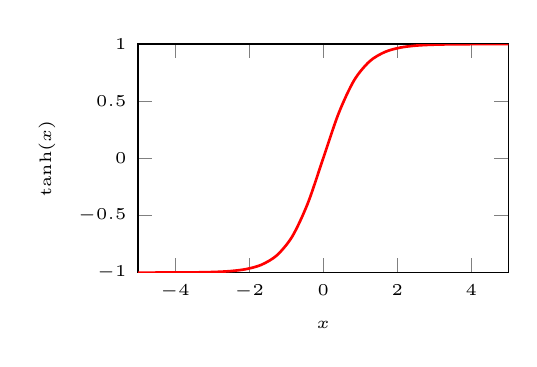
\begin{tikzpicture}[scale=1.2]
      \begin{axis}[width=5.5cm,height=4cm,
        ylabel=$\tanh(x)$,
        xlabel=$x$,ymin=-1,ymax=1,xmin=-5,xmax=5,
        style={font=\tiny\normalfont},
        legend style ={at={(0.5,1)},anchor=south,align=left}
        ]
        %\addplot[blue,smooth] {1/(1+exp(-x))};% \addlegendentry{Logistic sigmoid $\sigma(z)$}
        \addplot[thick,red,smooth] {tanh(x)}; %\addlegendentry{Hyperbolic tangent $\tanh(x)$}
        % \addplot[orange,smooth] {1/(1 + abs(x))}; \addlegendentry{Softsign $\fr{1}{1 + |z|}$}          
        % \addplot[green!50!black,smooth] {abs(tanh(x))}; \addlegendentry{Rectified hyperbolic tangent $|\tanh(z)|$}
        \end{axis}
      \end{tikzpicture}
      
    	% \caption[Sigmoidal activation functions.]{Common used activation functions include the logistic sigmoid $\sigma(z)$ and the hyperbolic tangent $tanh(z)$. More recently used activation functions are the softsign and the rectified hyperbolic tangent.}
    	% \label{fig:sigmoid-tanh}
    \end{figure}

  \item Preferred to sigmoid activation function due to its zero-centeredness.
    
  \end{itemize}
\end{frame}


\begin{frame}
  \frametitle{Rectified linear unit (ReLU)}
  \pause

  \begin{itemize}[<+->]
  \item The ReLU is given by
    \begin{equation}
      \text{ReLU}(x) = \pause \max(0,x)
    \end{equation}

  \item Performs a simple thresholding of input at 0.


    \begin{figure}[t!]\centering
      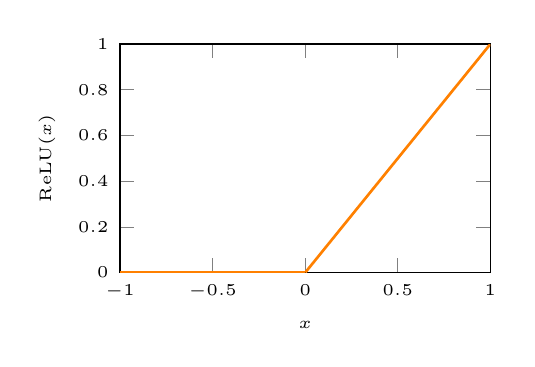
\begin{tikzpicture}[scale=1.2]
        \begin{axis}[width=5.5cm,height=4cm,
          ylabel=ReLU$(x)$,
          xlabel=$x$,ymin=0,ymax=1,xmin=-1,xmax=1,
          style={font=\tiny\normalfont},
          legend style ={at={(0.5,1)},anchor=south,align=left}
          ]
          % \addplot[blue,smooth] {1/(1+exp(-x))};% \addlegendentry{Logistic sigmoid $\sigma(z)$}
          \addplot[thick,orange,smooth,domain=-0.001:-1] {max(0,x)}; %\addlegendentry{Hyperbolic tangent $\tanh(x)$}
          \addplot[thick,orange,smooth,domain=0.001:1] {max(0,x)}; %\addlegendentry{Hyperbolic tangent $\tanh(x)$}
          % \addplot[orange,smooth] {1/(1 + abs(x))}; \addlegendentry{Softsign $\fr{1}{1 + |z|}$}          
          % \addplot[green!50!black,smooth] {abs(tanh(x))}; \addlegendentry{Rectified hyperbolic tangent $|\tanh(z)|$}
        \end{axis}
      \end{tikzpicture}
    \end{figure}

  \item Demonstrates faster convergence than $\bm\sigma(x)$ and $\tanh(x)$
  \item Popular for deep convolutional networks (several hidden layers)
  \item Neurons can be fragile, however, requiring care in selection of learning rate
  \end{itemize}
  
\end{frame}


 


\section{ANN operations}


\begin{frame}
  \frametitle{Neural network notation}
  \pause

  
  The sigmoid {\bf \bl activation (output)} of a neuron is denoted:\pause
  \begin{equation}\bl
    \bm\varphi(w_0z_1 + w_{1}z_2 + \cdots + w_{m-1} z_{m-1} + b) = \bm\varphi\lt(\sum w_iz_i + b\rt) = \text{new neuron}
  \end{equation}
  \pause
  Further, we denote each hidden unit as $z_{neuron}^{(layer)}$, e.g.\pause
  \begin{itemize}[<+->]
  \item $z_4^{(1)}$: fourth neuron in first layer (layers are counted from first hidden layer)
  \end{itemize}
  \pause

  \bigskip
  
  \begin{minipage}[t]{.47\linewidth}
  \textbf{\rd Weights} are denoted as $\rd w_{to,from}$, e.g.\pause
  \begin{itemize}[<+->]
  \item $w_{2,3}^2$: from the third neuron in the  layer 1 to the second neuron in layer 2
  \item The superscript is not often used, as it is clear from the context which layer we are dealing with
  \end{itemize}
\end{minipage}  \pause
\begin{minipage}[t]{.47\linewidth}
  \begin{figure}[h!]
    \centering
    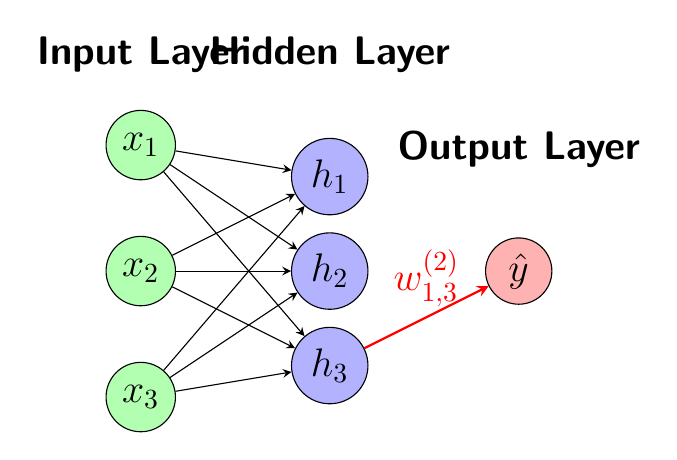
\begin{tikzpicture}[>=stealth,scale=0.8]
      % Input layer
      \node[circle,fill=green!30,draw] at (0,2) (x1) {$x_1$};
      \node[circle,fill=green!30,draw] at (0,0) (x2) {$x_2$};
      \node[circle,fill=green!30,draw] at (0,-2) (x3) {$x_3$};
      
      % Hidden layer with three units
      \node[circle,fill=blue!30,draw] at (3,1.5) (z1) {$h_1$};
      \node[circle,fill=blue!30,draw] at (3,0) (z2) {$h_2$};
      \node[circle,fill=blue!30,draw] at (3,-1.5) (z3) {$h_3$};
      
      % Output layer
      \node[circle,fill=red!30,draw] at (6,0) (y) {$\hat{y}$};
      
      % Connections from input to hidden
      \draw[->] (x1) -- (z1);
      \draw[->] (x1) -- (z2);
      \draw[->] (x1) -- (z3);
      \draw[->] (x2) -- (z1);
      \draw[->] (x2) -- (z2);
      \draw[->] (x2) -- (z3);
      \draw[->] (x3) -- (z1);
      \draw[->] (x3) -- (z2);
      \draw[->] (x3) -- (z3);
      
      % Connection from middle hidden unit to output
      \draw[->,thick,red] (z3) -- (y) node[midway,above] {$w_{1,3}^{(2)}$};
      
      % Layer labels
      \node[above] at (0,3) {Input Layer};
      \node[above] at (3,3) {Hidden Layer};
      \node[above] at (6,1.5) {Output Layer};
    \end{tikzpicture}
  \end{figure}
\end{minipage}
\end{frame}


\begin{frame}
  \frametitle{Matrix operations in neural networks}
  \pause
%  The activation in the next layer can be constructed as a matrix operation as follows.\pause

  Given the activation vector ($D$ neurons) in the zeroth (input) layer:
  \begin{equation}
   \bm x \in \mb{R}^D = \bm z^{(0)} =   \begin{bmatrix}
    z_1^{0}\\[2mm]
    z_2^{0}\\[2mm]
    \vdots \\[2mm]
    z_D^{0}\\
    \end{bmatrix}
  \end{equation}
  \pause
  Then the activations in the next layer ($M$ neurons) are given by:\pause
  \begin{equation}
    \bm{z}^{(1)}=
    \bm\varphi\left(
    \boldsymbol{W}\bm z^{(0)}+ \bm b
  \right)
  = \pause
  \bm\varphi \left(
    \begin{bmatrix}
      w_{1,1} & w_{1,2} & \cdots & w_{1,D}\\
      w_{2,1} & w_{2,2} & \cdots & w_{2,D}\\
      \vdots & \vdots & \ddots & \vdots \\
    w_{M,1} & w_{M,2} & \cdots & w_{M,D}\\
    \end{bmatrix}
    \, 
    \begin{bmatrix}
    z_1^{0}\\
    z_2^{0}\\
    \vdots \\
    z_{D}^{0}\\
    \end{bmatrix}
    +
    \begin{bmatrix}
    b_0\\
    b_1\\
    \vdots \\
    b_{M}\\
    \end{bmatrix}
    \right)
  \end{equation}
  \pause
  Example: If Layer 1 had only two neurons, then the weight matrix $\bm W$ would have only 2 rows.
\end{frame}


\begin{frame}
  \frametitle{ Example: MLP with two outputs}
  \pause

  This simple MLP has 2 layers (1 hidden, one outer), and 

  \begin{center}
  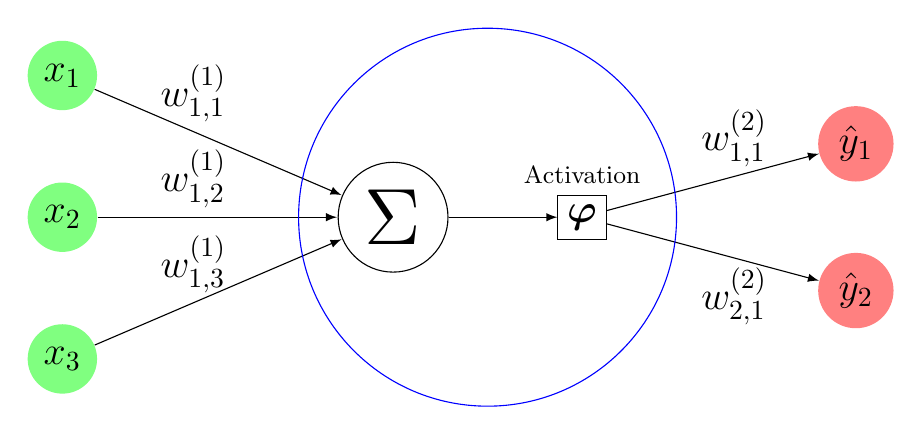
\begin{tikzpicture}[>=latex,scale=1.2]
\path
(0,0)     node[circle,draw,scale=2,inner sep=2pt] (S) {$\Sigma$}
% +(90:2.5) node[circle,draw,inner sep=2.5pt,opacity=0] (b) {}
%           node[above=1mm] {}
+(-3.5,1.5)  node[circle,fill=green!50]  (x1) {$x_1$}
+(-3.5,0)    node[circle,fill=green!50]  (x2) {$x_2$}
+(-3.5,-1.5) node[circle,fill=green!50]  (x3) {$x_3$}
(2,0)    node[draw] (g) {$\bm\varphi$} node[above=3mm]{\small\normalfont Activation}
+(15:3)  node[circle,fill=red!50]  (y1) {$\hat{y}_1$}
+(-15:3) node[circle,fill=red!50]  (y2) {$\hat{y}_2$};
\draw[->] (S)--(g);
%\draw[->] (b)--(S);
\draw[->] (g)--(y1) node[pos=.6,above]{$w_{1,1}^{(2)}$};
\draw[->] (g)--(y2) node[pos=.6,below]{$w_{2,1}^{(2)}$};
\draw[->] (x1)--(S) node[pos=.4,above]{$w_{1,1}^{(1)}$};
\draw[->] (x2)--(S) node[pos=.4,above]{$w_{1,2}^{(1)}$};
\draw[->] (x3)--(S) node[pos=.4,above]{$w_{1,3}^{(1)}$};
\draw[blue] (1,0) circle(2);
\end{tikzpicture}
\end{center}


\end{frame}



\begin{frame}[fragile]
   \frametitle{Example: 2-layer regression MLP }\pause  
    Two-layer MLP for regression \pause
    
    \begin{figure}
      \centering
      \begin{neuralnetwork}[height=4, nodespacing=1.7cm,layerspacing=5cm ]
      \newcommand{\x}[2]{$x_#2$}
      \newcommand{\y}[2]{$\hat{y}$}
      \newcommand{\hfirst}[2]{\small $z^{(1)}_{#2}$}
      \newcommand{\wfirst}[4]{\small $w^{(1)}_#2$}
      \newcommand{\mylinktext}[4]{$w^{(#3)}_{#4,#2}$}
      \newcommand{\hsecond}[2]{\small $h^{(2)}_{#2}$}
      \setdefaultlinklabel{\mylinktext}
      \visible<+->{\inputlayer[count=2, bias=false, text=\x]}
      \visible<+->{\hiddenlayer[count=4, bias=false,text=\hfirst]}
      %\visible<+->{\linklayers}
      \visible<+->{\link[from layer=0,to layer=1,from node=1,to node=1, labelpos=near end]}
      \visible<+->{\link[from layer=0,to layer=1,from node=1,to node=2, labelpos=near end]}
      \visible<+->{\link[from layer=0,to layer=1,from node=1,to node=3, labelpos=near end]}
      \visible<+->{\link[from layer=0,to layer=1,from node=1,to node=4, labelpos=near end]}
      \visible<+->{\link[from layer=0,to layer=1,from node=2,to node=1, labelpos= midway]}
      \visible<+->{\link[from layer=0,to layer=1,from node=2,to node=2, labelpos=midway]}
      \visible<+->{\link[from layer=0,to layer=1,from node=2,to node=3, labelpos=midway]}
      \visible<+->{\link[from layer=0,to layer=1,from node=2,to node=4, labelpos=midway]}
      \visible<+->{\outputlayer[count=1,text=\y]}
      \visible<+->{\linklayers}
    \end{neuralnetwork}
\end{figure}

  \end{frame}


\begin{frame}[fragile]
  \frametitle{Example: 2-layer regression MLP: scalar form equations}\pause  

  Given an observation $x_{nd}$ with $d= 1,\ldots, D$ features, \pause these equations describe the output from a 2-layer network:
  \pause
  
   \begin{eqnarray*}
    z_m^{(1)} &=& \bm\varphi\lt(\sum_{d=1}^{D} w_{1,d}^{(1)}x_{nd}  + b_d^{(1)} \rt)\\[2mm]\pause
    y_{i}(x_{i}) &=& \pause  \sum_{m=1}^{M} w_{1,m}^{(2)}z_m^{(1)}   + b^{(2)}   
  \end{eqnarray*}
  \pause
  %Note:
  \begin{itemize}[<+->]
  \item $D$ is number of input neurons
  \item $M$ is number of hidden neurons
  \item Total number of learnable parameters: \pause     $M(D+1)$ weights and $(D+1)$ biases
  \item Linear/identity activation is used in output
  \end{itemize}
 
\end{frame}


\begin{frame}
  \frametitle{Neural network loss function}
  \pause
  Given $K$ output neurons and $N$ observations (where   $f_k$ is the output),
  we can compute the loss (cost) functions $C$ as follows. \pause

  \medskip
  
  \textbf{For regression:}
  \begin{equation}
    \mc{L} = \pause \sum_{k=1}^K\sum_{n=1}^N(y_{nk} - f_k(x_n))^2
  \end{equation}

  \pause

  
  Thus, we can write, where $K=1$ (univariate output):

  \begin{equation}
        \mc{L} = \sum_{n=1}^N (y_n - \hat y_n)^2
  \end{equation}
  
  \medskip
  
  \textbf{For classification}, we use the cross-entropy (deviance) given $K$ classes:\pause
  \begin{equation}
       \mc{L} = - \sum_{n=1}^N\sum_{k=1}^Ky_{nk} \log f_k(x_n))
  \end{equation}

  \pause

\end{frame}

\begin{frame}
  \frametitle{Training a neural network}\pause
  
  \begin{itemize}[<+->]
  \item A neural network is trained or fitted by \textit{learning} the optimal values of the weights (and biases).
  \item This learning is done via optimization (e.g.\ gradient descent)
  \item Gradient descent update: \pause
    \begin{equation}
      w^{\text{new}} = w^{\text{old}} - \eta \pd{\mc{L}}{w^{\text{old}}}
    \end{equation}
    \pause
    where:
    \begin{itemize}[<+->]
    \item $\eta$ is the learning rate
    \item $\mc{L}$ is the cost function (e.g.\ residual sum of squares)
    \item $w$ the weight
  \end{itemize}

  \item In neural networks, the gradients are computed via \textbf{\bl backpropagation}
  \end{itemize}
\end{frame}




 
\section{Backpropagation}
\begin{frame}
  \frametitle{Backpropagation overview}

  \begin{figure}[h!]
    \centering

    \includegraphics<2->[width=.6\textwidth]{nn-complete}
  \end{figure}
\end{frame}


\begin{frame}
  \frametitle{Training procedure}\pause

  \begin{itemize}[<+->]
  \item Fix initial weights and perform a forward sweep/pass through the network computing the activations $a$ (outputs) of each layer $l$ as:\pause
    \begin{equation}
      \bm z^{(\ell)} = \bm \varphi(\bm W^{\ell} \bm z^{\ell-1} + \bm  b^{\ell})
    \end{equation}
  \item At the output layer, we compute the cost (loss) function $\mc L$ (what we want to minimize)
  \item Then, we {\it backpropagate} the errors through each layer in order to compute the gradients for the weight updates:\pause
    \begin{equation}
      \frac{\partial \mc{L}}{\partial \bm  W^{(L)}}
      =
      \frac{\partial \mc{L}}{\partial \bm z^{(L)}}
      \frac{\partial  \bm z^{(L)}}{\partial  \bm a^{(L)}}
      \frac{\partial  \bm a^{(L)}}{\partial  \bm W^{(L)}}
  \end{equation}
  \pause
  where $L$ is the last layer and $\bm a = \bm W \bm z^{\ell-1} + \bm b$
\item Repeat the forward and backward passes until cost is sufficiently minimized
  \end{itemize}
  
\end{frame}

\begin{frame}
  \frametitle{Equation summary: outer layer (regression case)}
  \pause
  At the outer layer $L$ (without indexing by neuron):\pause
  \begin{eqnarray}
    a^{(L)} &=& \bm w^{(L)\top} \bm z^{(L-1)} + b^{(L)} \\\pause
    o^{(L)} &=& a^{(L)}  \quad \text{(linear activation or {\it no} activation)} \\\pause
    \mc{L} &=& (o  - y)^2
  \end{eqnarray}
  \pause
  
  The gradient of the cost function with respect to $\bm w^{(L)}$ is:\pause
  \begin{equation}
    \frac{\partial \mc{L}}{\partial \bm w^{(L)}}
    =\pause
    \frac{\partial \mc{L}}{\partial  o}
    \frac{\partial o^{(L)}}{\partial a^{(L)}}
    \frac{\partial a^{(L)}}{\partial \bm w^{(L)}}
    =\pause
    2 \left(a^{(L)} - y \right) \bm z^{(L-1)}
  \end{equation}
  \pause
  Thus, we see that this gradient depends on the activation from the previous layer $a^{(L-1)}$. \pause Also wrt to the bias:
  \begin{equation}
    \pd{\mc{L}}{b^{(L)}} = \pause \pd{\mc{L}}{o}\pd{o}{a^{(L)}}\pd{a^{(L)}}{b^{(L)}} =\pause 2\lt(a^{(L)} - y\rt)(1)
  \end{equation}
\end{frame}

\begin{frame}
  \frametitle{Updating weights}
  \pause
  We can then update the weights for the last layer for the next iteration $r+1$:\pause
  \begin{eqnarray}
    w^{(L), r+1}  &=&  w^{(L),r} - \eta \pd{\mc{L}}{w^{(L)}}  \\\pause
    b^{(L), r+1}  &=&  b^{(L),r} - \eta \pd{\mc{L}}{b^{(L)}}  
  \end{eqnarray}
  \pause
  To update the weights for layer $L-1$, we need to find the gradients $\pd{\mc{L}}{w^{(L-1)}}$ and $\pd{\mc{L}}{b^{(L-1)}}$.

  \pause

  \medskip
  
  Using the chain rule again, we write:\pause
  \begin{eqnarray}
    \pd{\mc{L}}{w^{(L-1)}} &=& {\rd \pd{\mc{L}}{a^{(L-1)}}}\pd{a^{(L-1)}}{z^{(L-1)}}\pd{z^{(L-1)}}{w^{(L-1)}} \\\pause
    \pd{\mc{L}}{b^{(L-1)}} &=& {\rd \pd{\mc{L}}{a^{(L-1)}}}\pd{a^{(L-1)}}{z^{(L-1)}}\pd{z^{(L-1)}}{b^{(L-1)}} 
  \end{eqnarray}
\end{frame}

\begin{frame}
  \frametitle{Backward pass}
  \pause
  But we recall that $\mc{L}$ is not \textit{explicitly} dependent on $a^{(L-1)}$ as $C = (a^{(L)} - y)^2$.
  \pause

  However, it is \textit{implicitly} dependent, since\pause
  \begin{equation}
    C \propto a^{(L)},
  \end{equation}
  \pause
  \begin{equation}
    a^{(L)} \propto z^{(L)} 
  \end{equation}
  \pause
  and\pause
  \begin{equation}
    z^{(L)} \propto a^{(L-1)}
  \end{equation}
  \pause
  
  So, we use the chain rule to expand $\pd{\mc{L}}{a^{(L-1)}}$ as follows:\pause
  \begin{equation}\rd
    \pd{\mc{L}}{a^{(L-1)}} = \pause \pd{\mc{L}}{a^{(L)}}\pd{a^{(L)}}{z^{(L)}}\pd{z^{(L)}}{a^{(L-1)}}
  \end{equation}
\end{frame}

\begin{frame}
  \frametitle{Backward pass (cont.)}
  \pause
  We can then expand the cost function gradient wrt to weights for layer $L-1$ as:\pause
  \begin{eqnarray}
    \pd{\mc{L}}{w^{(L-1)}} &=& {\rd \pd{\mc{L}}{a^{(L-1)}}}\pd{a^{(L-1)}}{z^{(L-1)}}\pd{z^{(L-1)}}{w^{(L-1)}}
                          \\\pause
                        &=& {\rd \pd{\mc{L}}{a^{(L)}}\pd{a^{(L)}}{z^{(L)}}\pd{z^{(L)}}{a^{(L-1)}}} \pd{a^{(L-1)}}{z^{(L-1)}}\pd{z^{(L-1)}}{w^{(L-1)}} \\[2mm]\pause
    \pd{\mc{L}}{b^{(L-1)}} &=& {\rd \pd{\mc{L}}{a^{(L-1)}}}\pd{a^{(L-1)}}{z^{(L-1)}}\pd{z^{(L-1)}}{b^{(L-1)}}\\\pause                          
                           &=& {\rd \pd{\mc{L}}{a^{(L)}}\pd{a^{(L)}}{z^{(L)}}\pd{z^{(L)}}{a^{(L-1)}}} \pd{a^{(L-1)}}{z^{(L-1)}}\pd{z^{(L-1)}}{b^{(L-1)}} 
  \end{eqnarray}

  \pause

  Once these gradients are computed, we update the weights for the $(r+1)$th iteration using: \pause
   \begin{eqnarray}
    w^{(L-1), r+1}  &=& \pause  w^{(L-1),r} - \pause \eta \pd{\mc{L}}{w^{(L-1)}}  \\\pause
    b^{(L-1), r+1}  &=&  \pause b^{(L-1),r} - \pause \eta \pd{\mc{L}}{b^{(L-1)}}  
  \end{eqnarray}
\end{frame}

\begin{frame}
  \frametitle{Summary: forward pass}
  \begin{enumerate}[<+->]
  \item $(r=0)$: Initialize weights and biases: $w^{(l),0}$, $b^{(l),0}$
  \item Perform forward pass to compute activations:
    \begin{eqnarray}
      a^{(l),0} &=& w^{(l),0} \times z^{(l-1),0} + b^{(l),0} \\\pause
    z^{(l)} &=& \varphi(a^{(l),0}) 
    \end{eqnarray}
    \pause
    At output layer:
    \begin{eqnarray}      
      a^{(L),0} &=& w^{(L),0} \times z^{(L-1),0} + b^{(L),0} \\\pause
      o &=& \varphi(a^{(L),0}) \\
      C &=& (o  - y)^2
    \end{eqnarray}
  \end{enumerate}
\end{frame}

\begin{frame}
  \frametitle{Summary: backward pass---outer layer }
  \begin{enumerate}[<+->]\setcounter{enumi}{2}
  \item Backward pass, outer layer $(L)$:\pause
    \begin{enumerate}[<+->]
    \item Compute gradients: \pause
      \begin{eqnarray}
      \pd{\mc{L}}{w^{(L)}} &=& \pause \pd{\mc{L}}{o^{(L)}}\pd{o^{(L)}}{a^{(L)}}\pd{a^{(L)}}{w^{(L)}}\\\pause
      \pd{\mc{L}}{b^{(L)}} &=& \pause \pd{\mc{L}}{o^{(L)}}\pd{o^{(L)}}{a^{(L)}}\pd{a^{(L)}}{b^{(L)}}\pause
      \end{eqnarray}
    \item Update weights: \pause
      \begin{eqnarray}
        w^{(L), 1}  &=&  w^{(L),0} - \eta \pd{C^0}{w^{(L)}}  \\\pause
      b^{(L), 1}  &=&  b^{(L),0} - \eta \pd{C^0}{b^{(L)}}  
      \end{eqnarray}
  \end{enumerate}
  \end{enumerate}
\end{frame}

\begin{frame}
  \frametitle{Summary: backward pass---last hidden layer}
  \begin{enumerate}[<+->]\setcounter{enumi}{2}
  \item Backward pass, layer $(L-1)$:\pause
    \begin{enumerate}[<+->]\setcounter{enumii}{2}
    \item Compute gradients: \pause
    \begin{eqnarray}
      \pd{\mc{L}}{w^{(L-1)}} &=&  \pd{\mc{L}}{o^{(L)}}\pd{o^{(L)}}{a^{(L)}}\pd{a^{(L)}}{z^{(L-1)}}  \pd{z^{(L-1)}}{a^{(L-1)}}\pd{a^{(L-1)}}{w^{(L-1)}}\\\pause
      \pd{\mc{L}}{b^{(L-1)}} &=&   \pd{\mc{L}}{o^{(L)}}\pd{o^{(L)}}{a^{(L)}}\pd{a^{(L)}}{z^{(L-1)}}  \pd{z^{(L-1)}}{a^{(L-1)}}\pd{a^{(L-1)}}{b^{(L-1)}}
    \end{eqnarray}
    \pause
  \item Update weights: \pause
    \begin{eqnarray}
      w^{(L-1), 1}  &=& \pause  w^{(L-1),0} - \pause \eta \pd{\mc{L}}{w^{(L-1)}}  \\\pause
      b^{(L-1), 1}  &=&  \pause b^{(L-1),0} - \pause \eta \pd{\mc{L}}{b^{(L-1)}}  
    \end{eqnarray}
  \end{enumerate}
  \end{enumerate}
\end{frame}

\begin{frame}
  \frametitle{Summary: backward pass---second-to-last hidden layer}
  \begin{enumerate}[<+->]\setcounter{enumi}{2}
  \item Backward pass, layer $(L-2)$:\pause
    \begin{enumerate}[<+->] \setcounter{enumii}{4}
    \item Compute gradients: \pause
    \begin{eqnarray}
      \pd{\mc{L}}{w^{(L-2)}} &=&  \pd{\mc{L}}{o^{(L)}}\pd{o^{(L)}}{a^{(L)}}\pd{a^{(L)}}{z^{(L-1)}} \pause
                        \pd{z^{(L-1)}}{a^{(L-1)}}\pd{a^{(L-1)}}{z^{(L-2)}} \pause
                        \pd{z^{(L-2)}}{a^{(L-2)}}\pd{a^{(L-2)}}{w^{(L-2)}}\\\pause
      \pd{\mc{L}}{b^{(L-2)}} &=&   \pd{\mc{L}}{o^{(L)}}\pd{o^{(L)}}{a^{(L)}}\pd{a^{(L)}}{z^{(L-1)}} \pause
                        \pd{z^{(L-1)}}{a^{(L-1)}}\pd{a^{(L-1)}}{z^{(L-2)}} \pause
                        \pd{z^{(L-2)}}{b^{(L-2)}}\pd{a^{(L-2)}}{b^{(L-2)}}
    \end{eqnarray}
    \pause
  \item Update weights: \pause
    \begin{eqnarray}
      w^{(L-2), 1}  &=& \pause  w^{(L-2),0} - \pause \eta \pd{\mc{L}}{w^{(L-2)}}  \\\pause
      b^{(L-2), 1}  &=&  \pause b^{(L-2),0} - \pause \eta \pd{\mc{L}}{b^{(L-2)}}  
    \end{eqnarray}
  \end{enumerate}
  \end{enumerate}
\end{frame}


\begin{frame}
  \frametitle{Summary: backward pass---first hidden layer}
  \begin{enumerate}[<+->]\setcounter{enumi}{2}
  \item Backward pass, layer $(1)$:\pause
        \begin{enumerate}[<+->] \setcounter{enumii}{4}
    \item Compute gradients: \pause
    \begin{eqnarray}
      \pd{\mc{L}}{w^{(1)}} &=&  \pd{\mc{L}}{o^{(L)}}\pd{o^{(L)}}{a^{(L)}}\pd{a^{(L)}}{z^{(L-1)}}\pd{z^{(L-1)}}{a^{(L-1)}} \pause
                          \pause\cdots  
                          \pd{a^{(2)}}{z^{(1)}}\pd{z^{(1)}}{a^{(1)}}\pd{a^{(1)}}{w^{(1)}}\\\pause
      \pd{\mc{L}}{b^{(1)}} &=&  \pd{\mc{L}}{o^{(L)}}\pd{o^{(L)}}{a^{(L)}}\pd{a^{(L)}}{z^{(L-1)}}\pd{z^{(L-1)}}{a^{(L-1)}} \pause
                          \pause\cdots  
                          \pd{a^{(2)}}{z^{(1)}}\pd{z^{(1)}}{a^{(1)}}\pd{a^{(1)}}{b^{(1)}}
    \end{eqnarray}
    \pause
  \item Update weights: \pause
    \begin{eqnarray}
      w^{(1), 1}  &=& \pause  w^{(1),0} - \pause \eta \pd{\mc{L}}{w^{(1)}}  \\\pause
      b^{(1), 1}  &=&  \pause b^{(1),0} - \pause \eta \pd{\mc{L}}{b^{(1)}}  
    \end{eqnarray}
  \end{enumerate}
  \end{enumerate}
\end{frame}


\begin{frame}
  \frametitle{Summary of backpropagation}\pause

  \begin{enumerate}[<+->]
  \item Fix initial weights $w^{(l),0}$, $b^{(l),0}$ and perform a forward sweep/pass through the network computing the activations $a$ (outputs) of each layer $l$ as:\pause
    \begin{equation}
      a^{(l)} = \varphi(\bm W^{(l)} z^{(l-1)} + b^{(l)})
    \end{equation}
  \item At the output layer, we compute the cost function $C$ (what we want to minimize)
  \item Then, we {\it backpropagate} the errors through each layer in order to compute the gradients $\pd{\mc{L}}{w^{(l)}}$, $\pd{\mc{L}}{b^{(l)}}$ \pause
    and  weight updates  $w^{(l),r+1}$ and $b^{(l),r+1}$
\item Repeat the forward and backward passes until cost is sufficiently minimized
  \end{enumerate}
  
\end{frame}


\begin{frame}
  \frametitle{Example: backpropagation for 3-layer network}
  \pause
%  Consider the ANN below. What are the cost function gradients? \pause
\visible<2->{  \begin{figure}[h!]
    \centering
    \includegraphics[width=.6\textwidth]{4layer-nn}
  \end{figure}
}
\pause
\vspace{-2ex}
\begin{eqnarray}
 \pd{\mc{L}}{w^{(3)}} &=&  {\rd \pd{\mc{L}}{o^{(3)}}\pd{o^{(3)}}{a^{(3)}}} \pd{a^{(3)}}{w^{(3)}}\\\pause
 \pd{\mc{L}}{w^{(2)}} &=&  {\rd \pd{\mc{L}}{o^{(3)}}\pd{o^{(3)}}{a^{(3)}}}  {\bl \pd{a^{(3)}}{z^{(2)}}  \pd{z^{(2)}}{a^{(2)}}} \pd{a^{(2)}}{w^{(2)}} \\\pause
 \pd{\mc{L}}{w^{(1)}} &=&  {\rd \pd{\mc{L}}{o^{(3)}}\pd{o^{(3)}}{a^{(3)}}}  {\bl \pd{a^{(3)}}{z^{(2)}}  \pd{z^{(2)}}{a^{(2)}}}   \pd{a^{(2)}}{z^{(1)}} \pd{z^{(1)}}{a^{(1)}} \pd{a^{(1)}}{w^{(1)}}
\end{eqnarray}
\end{frame}



% \begin{frame}
%   \frametitle{Automatic differentiation}

%   Automatic differentiation (AD) is a set of techniques to numerically evaluate the derivative of a function specified by a computer program.

%   \medskip

%   \begin{itemize}[<+->]
%   \item AD exploits the fact that most functions are composed of elementary operations (addition, multiplication, etc.) for which derivatives are known.

%   \item There are two main modes of AD:
%     \begin{itemize}
%     \item Forward mode: propagates derivatives from inputs to outputs.
%     \item Reverse mode: propagates derivatives from outputs to inputs (used in backpropagation).
%     \end{itemize}
%   \end{itemize}

% \end{frame}

% \begin{frame}
%   \frametitle{Forward mode differentiation}\pause

%   Think of the output as a mapping $\bm o = \bm f(\bm x)$ where $\bm x \in\mathbb{R}^n$ and $\bm o \in\mathbb{R}^m$. \pause
%   Then
   
%   $\bm f$ is given by: \pause


%   \begin{equation}
%     \bm f = \bm f_4 \circ \bm f_3 \circ \bm f_2 \circ \bm f_1
%   \end{equation}
% \end{frame}



\section{Summary}

\begin{frame}
  \frametitle{Regression MLP architecture}
  \pause
  Typical hyperparameter values are: \pause

  \begin{table}\centering
  \begin{tabular}[t]{l l}
    \bf Hyperparameter & \bf Value \\\midrule
    \# input neurons & 1 per input feature \\[2mm]\pause
    \# hidden layers & Usually 1 -- 5 \\[2mm]\pause
    \# neurons per hidden layer & Usually 10 -- 100 \\[2mm]\pause
    \# output neurons & 1 per prediction dimension \\[2mm]\pause
    hidden layer activation & ReLU \\[2mm]\pause
    output activation & None (if unbounded) \\[2mm]\pause
    loss function & MSE or MAE/Huber
  \end{tabular}
\end{table}
\end{frame}

\begin{frame}
  \frametitle{Classification MLP architecture}
  \pause
  \begin{itemize}
  \item For classifcation, input and hidden layers are chosen in similar fashion to the regression case

    \pause

  \item However, the number of output neurons is given by the name of classes/labels

  \item The output layer activation is typically the softmax function:
    \begin{equation}
      \text{softmax}(z_{k}) = \fr{e^{z_{k}}}{\sum_{k'}e^{z_{k'}}}
    \end{equation}
    where $z_{k}$ is the unnormalized log probability of each class $k$
    
    \pause
    
  \item The loss function is taken as the cross entropy 
  \end{itemize}
\end{frame}

\begin{frame}
  \frametitle{Other types of neural networks}
  \pause

  The standard ANN architecture (MLP) we have studied is also called the feed-forward network.

  \medskip
  
  Other architectures have been shown to give better performance for various applications: \pause

  \medskip
  \begin{itemize}[<+->]
  \item Recurrent neural networks (RNNs): time-series forecasting

  \item Convolutional neural networks (CNNs): image classification

  \item Long short-term memory networks (LSTMs): time-series, pattern identification, etc.
  \end{itemize}

\end{frame}

\begin{frame}
  \frametitle{Reading}
 We will discuss the CNN on Wednesday, along with examples in Python.
 \begin{itemize}[<+->]
 \item \textbf{PMLI}: 13.1-3
 \item \textbf{PML}: 8.3, 9.4
 \item \textbf{ESL}: 11
 \item \textbf{DL}: 6-8, 11, 12 
 \item Experiment in this \href{http://playground.tensorflow.org}{\bl \bf playground}
  \end{itemize}
\end{frame}
 

\end{document}

%%% Local Variables:
%%% mode: latex
%%% TeX-master: t
%%% End:
